%%%%%%%%%%%%%%%%%%%%%%%%%%%%%%%%%%%%%%%%%%%%%%%
%
% Template per Elaborato di Laurea
% DISI - Dipartimento di Ingegneria e Scienza dell’Informazione
%
% update 2015-09-10
%
% Per la generazione corretta del 
% pdflatex nome_file.tex
% bibtex nome_file.aux
% pdflatex nome_file.tex
% pdflatex nome_file.tex
%
%%%%%%%%%%%%%%%%%%%%%%%%%%%%%%%%%%%%%%%%%%%%%%%

% formato FRONTE RETRO
\documentclass[epsfig,a4paper,11pt,titlepage,twoside,openany]{book}
\usepackage{epsfig}
\usepackage{plain}
\usepackage{setspace}
\usepackage[paperheight=29.7cm,paperwidth=21cm,outer=1.5cm,inner=2.5cm,top=2cm,bottom=2cm]{geometry} % per definizione layout
\usepackage{titlesec} % per formato custom dei titoli dei capitoli

\usepackage{hyperref}
\usepackage{amsmath}
\usepackage{nicefrac}
\usepackage[ruled,vlined]{algorithm2e}
\labelformat{algocf}{\textit{alg.}\,(#1)}

\SetKw{AND}{and}
\SetKw{OR}{or}
\SetKw{NOT}{not}
\SetKw{IN}{in}
\SetKw{DOWNTO}{downto}

\newcommand{\INTEGER}{\KwSty{int}}
\newcommand{\INTARRAY}{\INTEGER[\,]}
\newcommand{\SET}{\KwSty{set}}

\usepackage{url}
\usepackage{tikz}

\usepackage{circuitikz}
\usepackage{pgfplots}
\pgfplotsset{compat=1.17}
\usetikzlibrary{positioning, calc, arrows, automata, pgfplots.units}

\usepackage{minted} % Code

\usepackage{graphicx}
\graphicspath{ {./pictures} }

\definecolor{blue}{RGB}{22, 38, 77}
\definecolor{yellow}{RGB}{255, 236, 0}
\definecolor{orange}{RGB}{242, 145, 0}
\definecolor{red}{RGB}{173, 15, 10}

%%%%%%%%%%%%%%
% supporto lettere accentate
%
%\usepackage[latin1]{inputenc} % per Windows;
\usepackage[utf8x]{inputenc} % per Linux (richiede il pacchetto unicode);
%\usepackage[applemac]{inputenc} % per Mac.

\singlespacing

\usepackage[english]{babel}
\usepackage{csquotes}

\begin{document}

% nessuna numerazione
\pagenumbering{gobble}
\pagestyle{plain}

\thispagestyle{empty}

\begin{center}
  \begin{figure}[h!]
    \centerline{
\psfig{file=marchio_unitrento_colore_it_202002.eps,width=0.6\textwidth}}
  \end{figure}

  \vspace{2 cm} 

  \LARGE{Dipartimento di Ingegneria e Scienza dell’Informazione\\}

  \vspace{1 cm} 
  \Large{Corso di Laurea in\\
    ...
    %Informatica
    %Ingegneria dell'Informazione e delle Comunicazioni
    %Ingegneria dell'Informazione e Organizzazione d'Impresa
    %Ingegneria Elettronica e delle Telecomunicazioni
  }

  \vspace{2 cm} 
  \Large\textsc{Elaborato finale\\} 
  \vspace{1 cm} 
  \Huge\textsc{Titolo\\}
  \Large{\it{Sottotitolo (alcune volte lungo - opzionale)}}


  \vspace{2 cm} 
  \begin{tabular*}{\textwidth}{ c @{\extracolsep{\fill}} c }
  \Large{Supervisore} & \Large{Laureando}\\
  \Large{......}& \Large{......}\\
  \end{tabular*}

  \vspace{2 cm} 

  \Large{Anno accademico .../...}
  
\end{center}



\clearpage

%%%%%%%%%%%%%%%%%%%%%%%%%%%%%%%%%%%%%%%%%%%%%%%%%%%%%%%%%%%%%%%%%%%%%%%%%%
%%%%%%%%%%%%%%%%%%%%%%%%%%%%%%%%%%%%%%%%%%%%%%%%%%%%%%%%%%%%%%%%%%%%%%%%%%
%% Nota
%%%%%%%%%%%%%%%%%%%%%%%%%%%%%%%%%%%%%%%%%%%%%%%%%%%%%%%%%%%%%%%%%%%%%%%%%%
%% Sezione Ringraziamenti opzionale
%%%%%%%%%%%%%%%%%%%%%%%%%%%%%%%%%%%%%%%%%%%%%%%%%%%%%%%%%%%%%%%%%%%%%%%%%%
%%%%%%%%%%%%%%%%%%%%%%%%%%%%%%%%%%%%%%%%%%%%%%%%%%%%%%%%%%%%%%%%%%%%%%%%%%
%\thispagestyle{empty}

\begin{center}
  {\bf \Huge Ringraziamenti}
\end{center}

\vspace{4cm}


\emph{
  ...thanks to...
}

%\clearpage
\pagestyle{plain} % nessuna intestazione e pie pagina con numero al centro


% inizio numerazione pagine in numeri arabi
\mainmatter

%%%%%%%%%%%%%%%%%%%%%%%%%%%%%%%%%%%%%%%%%%%%%%%%%%%%%%%%%%%%%%%%%%%%%%%%%%
%%%%%%%%%%%%%%%%%%%%%%%%%%%%%%%%%%%%%%%%%%%%%%%%%%%%%%%%%%%%%%%%%%%%%%%%%%
%% Nota
%%%%%%%%%%%%%%%%%%%%%%%%%%%%%%%%%%%%%%%%%%%%%%%%%%%%%%%%%%%%%%%%%%%%%%%%%%
%% Si ricorda che il numero massimo di facciate e' 30.
%% Nel conteggio delle facciate sono incluse 
%%   indice
%%   sommario
%%   capitoli
%% Dal conteggio delle facciate sono escluse
%%   frontespizio
%%   ringraziamenti
%%   allegati    
%%%%%%%%%%%%%%%%%%%%%%%%%%%%%%%%%%%%%%%%%%%%%%%%%%%%%%%%%%%%%%%%%%%%%%%%%%
%%%%%%%%%%%%%%%%%%%%%%%%%%%%%%%%%%%%%%%%%%%%%%%%%%%%%%%%%%%%%%%%%%%%%%%%%%

% indice
\tableofcontents
\clearpage



% gruppo per definizone di successione capitoli senza interruzione di pagina
\begingroup
% nessuna interruzione di pagina tra capitoli
% ridefinizione dei comandi di clear page
\renewcommand{\cleardoublepage}{}
\renewcommand{\clearpage}{}
% redefinizione del formato del titolo del capitolo
% da formato
%   Capitolo X
%   Titolo capitolo
% a formato
%   X   Titolo capitolo

\titleformat{\chapter}
{\normalfont\Huge\bfseries}{\thechapter}{1em}{}

\titlespacing*{\chapter}{0pt}{0.59in}{0.02in}
\titlespacing*{\section}{0pt}{0.20in}{0.02in}
\titlespacing*{\subsection}{0pt}{0.10in}{0.02in}

% sommario
\chapter*{Abstract}
This thesis covers my work inside E-Agle Trento Racing Team from 2019 to 2021 as the lead firmware developer on the high-voltage battery management system for Fenice, the electric race car planned to compete in the 2022 Formula Student season. The paper overviews some key software components of the BMS that were introduced with my developments.

The first chapter introduces the competition environment and presents the team. The race organization and structure is explained to better understand the requirements of the car and the battery pack.

The introduction presents a simple overview of the powertrain of Fenice. It continues by explaining the basic behavior of batteries under load along with the physical and electrical structure of a battery pack. Requirements are then discussed on the capacity and maximum power of the pack. Finally the BMS architecture is overlaid and the role of each component is briefly explained.

The cell balancing algorithm is the topic of the third chapter. First, the problem is laid out with help from data acquired on the older car: Chimera Evoluzione. The balancing algorithm is then introduced along with all the requirements and constraints that justify the software design. Significant focus is put on the analysis of complexity of the algorithm.

A crucial element of the BMS, error management, is then analyzed. The chapter explains constraints imposed by the rulebook and the approach taken to respect them while having a scalable and efficient error tracking system that puts emphasis on timing accuracy and scheduling.

In conclusion the results of the cell balancing algorithm are shown with experimental data that validates the algorithm and its implementation. Some possible issues are identified and a fix is proposed.

The error management implementation is shown working on real hardware and the timing functionality is tested with the use of a logic analyzer.

A future advancement of the BMS in the form of state of charge estimation is then proposed, explaining the benefits of such a feature.

\newpage


%The last component covered in the thesis is the structure of an event-driven finite state machine library developed specifically for the needs of the BMS.

%This thesis covers my work on the development of a custom battery management system for a , with some references and comparisons to Chimera Evoluzione. This essay focuses on some key components of a BMS. The cell balancing algorithm, which maximizes usable battery energy by equalizing voltages between cells is discussed first. An overview of the algorithm, which overcomes hardware limitations to optimize the balancing process, will be the main focus of this chapter. Next, error management will be analyzed. Safety is the primary driving force behind most of the rulebook's rules on battery pack design and management. For this reason error management should be fast, precise and effective in all situations. A centralized management can prioritize errors based on severity, and provides a simple building block for many subsystems of the BMS. Lastly, an overview of the BMS architecture, with the main state machine and interaction between subsystems will be proposed.
%%%%%%%%%%%%%%%%%%%%%%%%%%%%%%%%%%%%%%%%%%%%%%%%%%%%%%%%%%%%%%%%%%%%%%%%%%
%%%%%%%%%%%%%%%%%%%%%%%%%%%%%%%%%%%%%%%%%%%%%%%%%%%%%%%%%%%%%%%%%%%%%%%%%%
%% Nota
%%%%%%%%%%%%%%%%%%%%%%%%%%%%%%%%%%%%%%%%%%%%%%%%%%%%%%%%%%%%%%%%%%%%%%%%%%
%% Sommario e' un breve riassunto del lavoro svolto dove si descrive 
%% l’obiettivo, l’oggetto della tesi, le metodologie e 
%% le tecniche usate, i dati elaborati e la spiegazione delle conclusioni 
%% alle quali siete arrivati.
%% Il sommario dell’elaborato consiste al massimo di 3 pagine e deve contenere le seguenti informazioni: 
%%   contesto e motivazioni
%%   breve riassunto del problema affrontato
%%   tecniche utilizzate e/o sviluppate
%%   risultati raggiunti, sottolineando il contributo personale del laureando/a
%%%%%%%%%%%%%%%%%%%%%%%%%%%%%%%%%%%%%%%%%%%%%%%%%%%%%%%%%%%%%%%%%%%%%%%%%%
%%%%%%%%%%%%%%%%%%%%%%%%%%%%%%%%%%%%%%%%%%%%%%%%%%%%%%%%%%%%%%%%%%%%%%%%%%      

%%%%%%%%%%%%%%%%%%%%%%%%%%%%%%%%
% lista dei capitoli
%
% \input oppure \include
%
\chapter{Background}

\section{Formula SAE}
Formula SAE is an international design competition founded by the American Society of Automotive Engineers (SAE) in 1980, in which university students develop, build and race an open-wheel, single-seater race car. The car must adhere to the Formula SAE rules that govern all the aspects of the car and the competition.

In Europe, Formula Student Germany (FSG) is the main governing body. FSG releases the rulebook \cite{fsg2020} that is used in all European competitions and it organizes the biggest competition of the season. Many more Formula SAE events are held all around Europe and the world.

\subsection{Competitions}
A Formula SAE competition consists of static and dynamic events in which industry experts judge the cars and the teams on several different aspects by awarding points for each event.

\subsubsection{Tech Inspections}
At the start of the competition technical inspections are carried out to verify that each car is respecting the rulebook and is thus eligible to participate in the dynamic events.
The inspection is carried out as follows:
\begin{itemize}
    \item \textbf{Pre-inspection}: safety hardware, driver equipment, tires, and rims are checked for compliance with the SAE and FIA rules.
    \item \textbf{Accumulator inspection}: the battery pack's adherence to the SAE rules is verified by checking its insulation and data acquisition methods. The pack is then sealed for the rest of the competition.
    \item \textbf{Electrical inspection}: all electrical components on the car are checked for compliance by verifying every component's datasheet. Furthermore, electrical grounding is checked all across the car.
    \item \textbf{Mechanical inspection}: It is verified that the car's dimensions are within rulebook specification. All strength samples for the chassis materials are shown to the officials.
    \item \textbf{Tilt test}: the car with the driver is put on an inclined platform with a lateral angle of 60 degrees. The car must adhere to the platform's surface and no fluids must leak.
    \item \textbf{Rain test}: the car is sprinkled with water for 120s to check proper humidity insulation of electronic components. The car must be on during the test and must remain powered for an additional 120 s.
    \item \textbf{Brake test}: the driver accelerates the car, switches it off and performs an emergency brake test. All four wheels must lock and the car must not deviate its path.
\end{itemize}
If the car passes every step of the tech inspections, it gets certified and can participate in the dynamic events.

\subsubsection{Static Events}
In static events, the car and the team are evaluated on theoretical points including design processes, team organization, business ideas, and more.
Static events are divided into three separate categories:
\begin{itemize}
    \item \textbf{Engineering design} (150 pts.): The judges evaluate the whole design process of the car, from the early stages of evaluation to the realization and validation of components. Each team's department has to justify all choices made in the design phase with data collected from simulations, previous experience, or QFD methodology.
    \item \textbf{Cost and manufacturing} (100 pts.): The team provides an engineering and a manufacturing BOM in which the cost of each component is reported. Team members have to explain the cost of every component, material, and manufacturing process.
    \item \textbf{Business plan presentation} (100 pts.): In the business plan presentation judges pretend to be potential investors and the team has to make an enticing presentation of its product and the business model in which the team plans to mass-produce the prototype car with studies on costs and profitability. Innovative and original ideas are usually rewarded.
\end{itemize}

\subsubsection{Dynamic Events}
Dynamic events value the overall performance of the car compared to its competitors. The car is put through four different tests that each assesses a different aspect of performance:
\begin{itemize}
    \item \textbf{Skidpad} (75 pts.): the car must complete two laps of a figure 8 track, sometimes on wet tarmac.
    \item \textbf{Acceleration} (75 pts.): the car must do a standing start and complete a straight 75 m long track as fast as possible.
    \item \textbf{Autocross} (100 pts.): a single lap of an autocross track with a length lower than 1,5 km must be completed in the least time possible. The track contains slaloms, straights, and sharp turns.
    \item \textbf{Endurance and efficiency} (425 pts.): the car must race for a total length of 22 km around a track similar to the autocross layout.
\end{itemize}
For each of the previous events, points are calculated based on the time taken to complete the race. For the Endurance event efficiency is also taken into account.

\section{E-Agle Trento Racing Team}
E-Agle Trento Racing Team is the Formula SAE team of the University of Trento. The team was created in 2016, and was immediately involved in the creation of electric race cars. Since its inception, the team realized two Formula SAE cars: Chimera and Chimera Evoluzione. Instead of following an evolutionary approach with the third car, the team decided to design the vehicle from scratch. This choice came from the experience with the two previous cars: some inconvenient design flaws and the will to innovate were the main driving forces of this decision.

The redesign was completed in 2019 with production planned to end in time for the 2020 racing season; unfortunately, due to the COVID-19 pandemic, all competitions were canceled and the team was forced to work away from the workshop. In 2021 production was resumed and the car is planned to compete in the second half of the 2021 season and continue for 2022.

The team is divided into four main divisions, each in charge of a different assembly of the car:
\begin{itemize}
    \item \textbf{Mechanical Team}: is in charge of the design, manufacturing and testing of every mechanical component of the car including the chassis, suspension components, aerodynamics and more.
    \item \textbf{Dynamics and Modeling Team}: the team develops the suspension kinematics and the whole car dynamics based on simulations of a virtual model of the car. By using the same model the team then creates the control logic of the vehicle that includes the traction control and torque vectoring algorithms.
    \item \textbf{Electronics Team}: Fenice relies on custom-designed electronics for most of its features. The team's job is to design and test all the electronic components, from the car's wiring to the high-voltage battery pack, from the printed circuit boards to the complex battery management system inside the high-voltage battery.
    \item \textbf{Software Team}: The award-winning cockpit HMI embedded in the steering wheel is fully custom built by the software team along with the telemetry system that provides data logging and live telemetry. In addition, the team is responsible for developing the control boards designed by the electronics division.
\end{itemize}

\begin{figure*}[h]
    \centering
    \includegraphics[width=\textwidth]{fenice}
    \caption{A render of Fenice}
    \label{fig:fenice_render}
\end{figure*}

\newpage


\chapter{Introduction}
\label{cha:intro}
A battery management system is a safety-critical component of modern battery packs. Especially in an automotive environment, where electric vehicle batteries can be subject to unoptimal working conditions, the need of a control system that ensures that the battery operates safely and efficiently is necessary.

\section{Formula SAE}
Formula SAE is an international design competition founded by the Society of Automotive Engineers in 1980, in which university students have to develop, build and race an open-wheel, single seater race car.\\
In Europe, Formula Student Germany releases the rulebook \cite{fsg2020} that delineates how a Formula SAE car should be constructed to be eligible to participate in european competitions.
TODO: battery rules here?\\

\section{Tractive System}
\begin{figure}[h]
    \centering
    \ctikzset{bipoles/crossing/size=.6}
\begin{circuitikz} \draw
    (0,1) to[battery=\(BAT\)] ++(0,3)

    (0,4) to[nos=\(AIR-\), n=airm] ++(5,0)
    to (5, 2.6) -- ++(2,0) -- (7, 4.5) -- ++(1.5,0)
    (7, 2.4) -- (7.75,2.4) -- (7.75,3.5) -- (8.5,3.5)
    (8.5,4.5) to[C=\(C_1\)] (8.5,3.5)

    (0,1) to[nos=\(AIR+\), n=airp] ++(5,0)
    to (5,2.4) -- ++(2,0) -- (7, 0.5) -- ++(1.5,0)
    (7, 2.6) to[crossing] ++(1.5,0) -- (8.5,1.5)
    (8.5,1.5) to[C=\(C_2\)] (8.5,0.5)

    (0.5,1) -- ++(0,-1)
    to[nos=\(S_p\),n=pre_sw] ++(2, 0)
    to[R=\(R_p\),n=pre_sw] ++(2,0)
    to ++ (0,+1)

    (8.5,0.5) edge[dashed] ++(1,0)
    (8.5,1.5) edge[dashed] ++(1,0)

    (8.5,3.5) edge[dashed] ++(1,0)
    (8.5,4.5) edge[dashed] ++(1,0)

    {[anchor=north] (6,2.4) node {\(Bus_+\)} [anchor=south] (6,2.6) node {\(Bus_-\)}};

    \draw (11.5,3.75) node[elmech](M1){M1}
    (9.75,4.9) -- ++(1,0) -/ (M1.150)
    (9.75,3.75) -| (M1.180)
    (9.75,2.65) -- ++(1,0) -/ (M1.210)
    ;
    \draw (11.5,1.25) node[elmech](M2){M2}
    (9.75,2.35) -- ++(1,0) -/ (M2.150)
    (9.75,1.25) -| (M2.180)
    (9.75,0.1) -- ++(1,0) -/ (M2.210)
    ;

    \draw[dotted] (-2,5) rectangle (5.25,-0.5) node[at start, right, fill=white] {Pack};
    \draw[dashed] (6.75,5) rectangle (9.75,2.55) node[at start, right, fill=white] {Inverter 1};
    \draw[dashed] (6.75,0) rectangle (9.75,2.45) node[at start, right, fill=white] {Inverter 2};
\end{circuitikz}
    \caption{Tractive system block schema}
    \label{fig:tractive_system}
\end{figure}

The tractive system is the whole high-voltage system of the car. It comprises the battery pack, the inverters and the electric motors that drive the wheels of the car.
The E-Agle TRT's car is powered by two independent three-phase permanent-magnet motors that drive the rear wheels of the car.

\section{Battery Architecture}
TODO: add circuits\\
A battery is an electrical energy storage system that relies on chemical reactions to generate a voltage. The main properties of a battery are: nominal voltage, internal resistance, energy capacity and discharge rate.\\
The voltage of a battery is influenced by many factors including: state of charge, temperature and applied load.\ The open-circuit voltage of a Lithium-Ion battery cell is 4.2V at 100\% state of charge and 3.0V at 0\%.
When a load is applied to a cell, the voltage drops according to Ohm's law: $V_{dropped} = R_{internal}*I_{load}$.

\subsection{Battery Pack}
A battery pack is a group of cells connected in series and parallel to form a bigger battery. Arranging the cells in series means that the current will only travel down a single path, passing through every cell. In this case the potential of each cell is summed. \\
In a parallel arrangement, electrons travel down multiple paths, splitting the current across more cells. This increases the current output of the battery, but the voltage is kept equals to a single cell's.\ A parallel connection of cells is also called a module, as it can be seen as a single, bigger battery cell.
The structure of a battery pack is based on it's specific application. For example, if high voltage was to be requested, the battery would have had many modules in series whereas, if the application required an high power output or larger capacity, more cells in parallel would be arranged.

In a Formula SAE car, the optimal setup is a lightweight, high-voltage and high-power battery pack. The rulebook limits voltage to 600V \cite[EV 4.1.1]{fsg2020} and power to 80kW \cite[EV 2.2.1]{fsg2020}, so the resulting battery will have as many cells in series as permitted and as little parallels as needed to reach the required power and capacity target. E-Agle TRT car's pack features 108 cells in series and only 4 in parallel, for a total of 432 cells and \~{}388V of nominal voltage (3.6V per cell). The high power requirement is fullfilled by the use of high-discharge rate cells, 45A in this case that result in an output  of 180A of continuous discharge current. As a consequence, The maximum theoretical power output is \~{}70kW and the energy capacity amounts to 6.2kWh.

\begin{figure}[h]
    \centering
    \begin{circuitikz}
    % Cell
    \draw (0,2) to[battery1] (0,3);
    \draw node[circle,draw,anchor=center,scale=4,label=Cell] (cell) at (0,2.5) {};

    % Cell to Module
    \draw node[circle,draw,anchor=center,scale=2.5] (ctm) at(2.25,2.5) {};
    \draw[->] (cell.east) -- (ctm.west);

    % Module
    \draw (2.75,1.5) -- ++(0,0.5) -| ++(-0.5,0) to[battery1] ++(0,1) -| ++(0.5,0.5)
    (2.75,2) -- ++(0.5,0) to[battery1] ++(0,1) -- ++(-0.5,0);
    \draw (3.25,2) edge[dotted] ++(0.5,0)
    (3.25,3) edge[dotted] ++(0.5,0);
    \draw node[circle,draw,anchor=center,scale=7,label=Module] (module) at (2.75,2.5) {};

    % Module to Block
    \draw node[circle,draw,anchor=center,scale=2.5] (mtb) at(6.5,2.5) {};
    \draw[->] (module.east) -- (mtb.west);

    % Block
    \draw (6.5,1) to[battery1] ++(0,1) to[battery1] ++(0,1) to[battery1] ++(0,1);
    \draw node[circle,draw,anchor=center,scale=9,label=Block] (block) at (6.5,2.5) {};

    % Block to Segment
    \draw[->] (block.east) -- (9.65,2.5);

    % Segment
    \draw (9.625,3) -- ++(0,+0.25);
    % 1
    \draw[solid] (9.5,2) rectangle ++(0.25,1);
    \draw (9.625,2) -- ++(0,-0.25) -| ++(0.5,0.25) ;
    % 2
    \draw[solid] (10,2) rectangle ++(0.25,1);
    \draw (10.125,3) -- ++(0,0.25) -| ++(0.5,-0.25) ;
    % 3
    \draw[solid] (10.5,2) rectangle ++(0.25,1);
    \draw (10.625,2) -- ++(0,-0.25) -| ++(0.5,0.25) ;
    % 4
    \draw[solid] (11,2) rectangle ++(0.25,1);
    \draw (11.125,3) -- ++(0,0.25) -| ++(0.5,-0.25) ;
    % 5
    \draw[solid] (11.5,2) rectangle ++(0.25,1);
    \draw (11.625,2) -- ++(0,-0.25) -| ++(0.5,0.25) ;
    % 6
    \draw[solid] (12,2) rectangle ++(0.25,1);
    \draw (12.125,3) -- ++(0,0.25);

    \draw node[circle,draw,anchor=center,scale=10,label=Segment] (segment) at (10.825,2.5) {};

    % Segment to Pack
    \draw[->] (segment.east) -- (14.15,2.5);

    % Pack
    \draw (14.125,3) -- ++(0,+0.25);
    % 1
    \draw[solid] (14,2) rectangle ++(0.25,1);
    \draw (14.125,2) -- ++(0,-0.25) -| ++(0.5,0.25) ;
    % 2
    \draw[solid] (14.5,2) rectangle ++(0.25,1);
    \draw (14.625,3) -- ++(0,0.25) -| ++(0.5,-0.25) ;
    % 3
    \draw[solid] (15,2) rectangle ++(0.25,1);
    \draw (15.125,2) -- ++(0,-0.25) -| ++(0.5,0.25) ;
    % 4
    \draw[solid] (15.5,2) rectangle ++(0.25,1);
    \draw (15.625,3) -- ++(0,0.25) -| ++(0.5,-0.25) ;
    % 5
    \draw[solid] (16,2) rectangle ++(0.25,1);
    \draw (16.125,2) -- ++(0,-0.25) -| ++(0.5,0.25) ;
    % 6
    \draw[solid] (16.5,2) rectangle ++(0.25,1);
    \draw (16.625,3) -- ++(0,0.25);

    \draw node[circle,draw,anchor=center,scale=10,label=Pack] (pack) at (15.4,2.5) {};

\end{circuitikz}
    \caption{Battery pack elements naming scheme}
    \label{fig:naming}
\end{figure}
As explained in figure \ref{fig:naming}, the pack is subdivided in parts that can be summarised as follows:
\begin{itemize}
    \item A cell is the basic unit of a battery pack.
    \item A parallel of four cells forms a module (also called cell in some cases).
    \item Blocks are a series of three modules, that are mounted in a single physical element.
    \item The rulebook mandates the separation of the pack into smaller segments with precise characteristics \cite[EV 5.3.2]{fsg2020}. In this case a segment is a series of six blocks, totalling a maximum voltage of 75.6V and \~1.2kWh of energy, below the limit of 120V and 1.6 kWh.
    \item Finally, the battery pack is a collection of six segments in series.
\end{itemize}

\subsection{Internal Connections}
To better control the pack, two Accumulator Isolation Relays (AIR) \cite[EV 5.6]{fsg2020} are located at both poles of the pack to disconnect its output when not needed. These relays are controlled by the BMS and can also be switched off by external devices such as emergency buttons located around the car.
\begin{figure}[h]
    \centering
    \ctikzset{bipoles/crossing/size=.6}
\begin{circuitikz} \draw
    (0,1) to[battery=\(BAT\),american] ++(0,3)

    %% Negative battery bus
    (0,4) to[fuse=\(F\)] ++(1.5,0) to[nos=\(AIR-\), n=airm] ++(2,0) -- ++(1.5,0)
    -- (5, 2.6) to[short, -*] ++(2,0) -- (7, 4.5) -- ++(1.5,0)

    %% Inverter 1
    (7, 2.4) to[short, *-] (7.75,2.4) -- (7.75,3.5) -- (8.5,3.5)
    (8.5,3.5) to[C=\(C_1\), n=c1, *-*] (8.5,4.5)

    (8.5,0.5) -- ++(0.75,0)
    (8.5,1.5) -- ++(0.75,0);
    \draw[solid] (9.25,3.25) rectangle ++(0.5,1.5);
    \path (9.25,3.25) -- ++(0,-0.5);
    \draw[dotted] (7.3,5) rectangle (10,3) node[at start, right, fill=white] {Inverter 1};

    %% Positive battery bus
    \draw (0,1) to[nos=\(AIR+\), n=airp] ++(5,0)
    to (5,2.4) -- ++(2,0) -- (7, 0.5) -- ++(1.5,0)

    %% Inverter 2
    (7, 2.6) to[crossing] ++(1.5,0) -- (8.5,1.5)
    (8.5,0.5) to[C=\(C_2\), *-*] (8.5,1.5)

    (8.5,3.5) -- ++(0.75,0)
    (8.5,4.5) -- ++(0.75,0);
    \draw[solid] (9.25,1.75) rectangle ++(0.5,-1.5);
    \draw[dotted] (7.3,0) rectangle (10,2) node[at start, right, fill=white] {Inverter 2};

    %% Pre-charge circuit
    \draw (0.5,1) to[short, *-] ++(0,-1)
    to[nos=\(S_p\),n=pre_sw] ++(2, 0)
    to[R=\(R_p\),n=pre_sw] ++(2,0)
    to[short, -*] ++(0,+1)

    {[anchor=north] (6,2.4) node {\(Bus_+\)} [anchor=south] (6,2.6) node {\(Bus_-\)}};

    %% Motor 1
    \draw (11,4) node[elmech](M1){M1}
    (9.75,4.65) -- ++(0.75,0) -- (M1.150)
    (9.75,4) -| (M1.180)
    (9.75,3.35) -- ++(0.75,0) -- (M1.210)
    ;

    %% Motor 2
    \draw (11,1) node[elmech](M2){M2}
    (9.75,1.65) -- ++(0.75,0) -/ (M2.150)
    (9.75,1) -| (M2.180)
    (9.75,0.35) -- ++(0.75,0) -/ (M2.210)
    ;

    \draw[dotted] (-2,5) rectangle (5.25,-0.5) node[at start, right, fill=white] {Battery Pack};


\end{circuitikz}
    \caption{Tractive system schema}
    \label{fig:tractive_system_detail}
\end{figure}

\section{Battery Management}
Battery management is a collection of operations that ensure the safety and efficiency of the battery pack's operation.\\
A battery management system should constantly measure cell temperatures, module voltages along with the total pack current output and check that each of those values is within specification. If anomalies are detected, the battery should be disconnected immediately.

\section {Module Balancing}
Cells are not perfectly identical and can have slight variations in internal resistance between each other. These imperfections mean that after some use, modules can start to deviate in voltage output between one another. This poses a limitation on the depth at wich the battery can be charged or discharged, reducing the total usable capacity of the pack.\\
Solving this problem involves charging or discharging every module until they all are inside an acceptable threshold.\\
Example:
TODO: module voltages chart and explanation


\chapter{Cell Balancing}
\label{cha:balancing}
As discussed in the introduction, the problem of battery balancing can reduce net battery capacity. To realize the extent of the losses, Chimera Evoluzione's battery pack has been analyzed. Chimera Evoluzione did not feature cell balancing, but could still measure individual cell voltages and has been in use for one year without being manually balanced. \autoref{fig:chimera_imbalance} shows measured open-circuit voltages of the whole battery pack.

\begin{figure}[h]
    \centering
    \begin{tikzpicture}
    \begin{axis}[
            width=12cm,
            enlargelimits=0.02,
            xlabel=Cell number,
            ybar interval,
            ylabel=Voltage,
            xtick={0,18,36,...,108},
            bar width=4pt
        ]
        \addplot [draw=red,fill=red!60] table[x=index,y=voltage, col sep=comma]{pictures/chimera_imbalance.csv};
    \end{axis}
\end{tikzpicture}
    \caption{Unbalanced Chimera Evoluzione cells.}
    \label{fig:chimera_imbalance}
\end{figure}

As can be seen in the chart, The difference between the highest-voltage cell ($V_{max} = V_{70} = 3.712 V$) and the lowest-voltage cell ($V_{min} = V_{73} = 3.554 V$) is $V_{delta}=V_{max}-V_{min}=0.158 V$. The difference between the average voltage and the minimum and maximum voltage is respectively $V^0_{delta} = V_{avg} - V_{min} = 0.066 V$ and $V^1_{delta} = V_{max} - V_{avg} = 0.091 V$.

If the pack in those conditions is discharged until $V_{73}$ reaches the cut-off voltage of $V_{low} = 3.000 V$, the average cell voltage would be $V^0_{avg} = V_{low} + V^0_{delta} = 3.066 V $. Similarly, if the battery is charged until $V_{70}$ reaches $V_{high} = 4.200 V$, the average voltage could only reach $V^1_{avg} = V_{high} - V^1_{delta} = 4.109 V$.

Chimera Evoluzione's battery pack is a 108s6p design, with each cell rated at 9.36 Wh nominal. Considering the discharge capacity curve for a single cell at 5 A \autoref{chap:vtc5}, the capacity lost between $V_{high}$ and $V^1_{avg}$ can be approximated to 0.2 Wh, or 2.1\% of a cell's energy. The low-end capacity between $V_{low}$ and $V^0_{avg} = 3.0 V$ is close to 0.2 Wh as well. Assuming a total pack nominal energy capacity of $E_{total} = 6065.3 Wh$, the energy loss amounts to $E_{lost} = E_{total}*4.2\% = 255 Wh$. Assuming a usable capacity of $E_{total}$ during an endurance event the average energy consumption of the car should remain below $\nicefrac{E_{total}}{22 km}=275\nicefrac{Wh}{km}$ without a safety margin. If a 10\% margin is considered, the maximum consumption is $C_{max} = 248\nicefrac{Wh}{km}$. It can then be assumed that the cost of an unbalanced battery pack is $\Delta S = \nicefrac{E_{lost}}{C_{max}} = 1 km$ of range in an endurance event.

With the use of cell balancing, it is expected to get imbalance values below 10 mV between all cells, making losses irrelevant.

\section{Balancing techniques}
There are different methods to balance a battery pack; They can be summarized into passive balancing, energy transfer and individual charge control \cite{6966514}.
Passive balancing is the simplest technique to implement: it only needs a switched shunt resistor in parallel to each battery module that dissipates the excess energy from each cell. The main disadvantages are the great heat generation that requires active cooling and the reduced overall efficiency of the battery pack that loses some of its energy through the balancing process.
\begin{figure}[h]
    \centering
    
\includegraphics[scale=1.5]{passive_balancing.png}
    \caption{Passive balancing wiring schema}
    \label{fig:passive_balancing}
\end{figure}

More efficient techniques exist under the name of active balancing. As the name suggests, excess energy is not wasted using these methods.
Energy transfer is a balancing strategy that can move energy between cells of the pack. For this to work, every cell must be interconnected with each other with some circuitry. One of the simplest transfer circuits is made of capacitors that can be alternately connected in parallel to two adjacent cells. Both poles of each capacitor can be switched at the same time to be connected to either one of the two cells, charging the capacitor from one cell and discharging it on the other, using the capacitor as a bucket to transfer energy between the cells. This is the simplest active balancing method, but its simplicity has the disadvantage of being slow to transfer energy between distant cells \cite{6966514}. More capacitor tiers can be added to provide more transfer paths at the cost of scalability.

Other systems with increased complexity involve the use of transformers, buck-boost converters or more complicated methods to transfer energy between each cell with more flexibility.

In the use case of a Formula SAE car, where the battery goes through full charge and discharge cycles, the disadvantages of a passive solution are less relevant, while the increased complexity of active balancing results in more weight and failure points. If done only during charging, passive balancing doesn't affect the running efficiency of the car, as it doesn't discharge cells when the car is running. Active balancing could provide efficiency advantages if the battery doesn't get fully charged often, as happens in road cars. For these reasons, a passive balancing design was chosen.

More advanced balancing algorithms base the imbalance computation on the state of charge of the cell instead of cell voltage \cite{8834858}. This preliminary study focuses on voltage values as a reference, since the state of charge estimation is not yet implemented in the BMS.

The balancing hardware is located on the cellboards and is composed of the battery management chip that drives external transistors which can connect each battery module in parallel with a power resistor. The resulting circuit discharges the module at a rate of $400 mA$ \cite{fenice-bms-hv}.

\subsection{Strategy}
A design constraint in the balancing circuitry on the cellboards prevents two adjacent cells to be discharged simultaneously. To work around this problem an algorithm has been developed to select the optimal set of cells that can be discharged at the same time.

\begin{figure}[h]
    \centering
    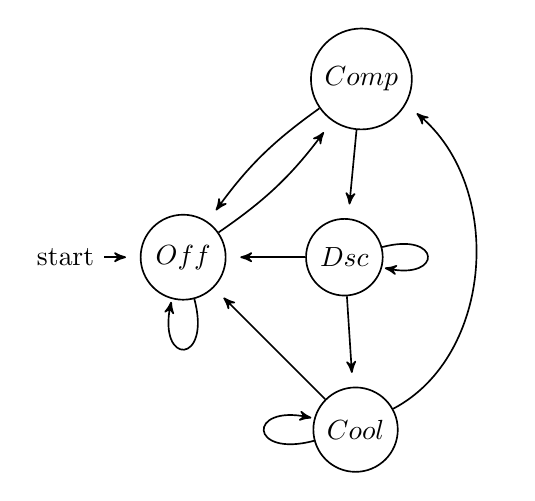
\begin{tikzpicture}[->, >=stealth', shorten >= 5pt, node  distance = 2.5cm, semithick]
	\node[state, initial]	(off)                         {$Off$};
	\node[state]            (computing)      [above right=2cm of off]          {$Comp$};
	\node[state]            (discharging)  [right=1cm of off]                 {$Dsc$};
	\node[state]            (cooldown)   [below right=2cm of off]           {$Cool$};

	\path (off)      edge[bend right=10] (computing)
	edge[loop below] (off);
	\path (computing) edge (discharging)
	edge [bend right=10] (off);
	\path (discharging) edge[loop right] (discharging)
	edge (cooldown)
	edge(off);
	\path (cooldown) edge[loop left] (cooldown)
	edge[bend right=60] (computing)
	edge(off);
	%\path (pc_start)    edge (pc_wait);
	%\path (pc_wait)     edge[loop below] (pc_wait)
	%edge[bend left=5] (ts_off)
	%edge (pc_end);
	%\path (pc_end)      edge[bend left=10] (ts_on)
	%edge[bend right=10] (charge);
	%\path (ts_on)       edge[loop right] (ts_on)
	%edge[bend right=7] (ts_off);
	%\path (charge)      edge[loop left] (charge)
	%edge[bend right] (ts_off);
	%\path (stacca)      edge (halt);
	%\path (halt)        edge[loop left] (halt);
	%\path (all)         edge (stacca);
\end{tikzpicture}

    \caption{Balancing state machine}
    \label{fig:bms_fsm}
\end{figure}

When enabled, the cell balancing algorithm runs periodically following the state machine shown in \autoref{fig:bms_fsm}: first, the algorithm computes the set of cells to discharge (\textit{Comp}); The balancing ICs on the cellboards are then instructed to start the discharge process on selected cells. The discharge period lasts 30 seconds at the end of which there is a cooldown period of 10 seconds, which lets the voltages stabilize and the discharge resistors cool down. After cooldown, the algorithm is executed again. If no cells need discharging anymore, the state machine goes back to the \textit{Off} state. The balancing state machine can be stopped at all times by external events.
%Cell balancing is divided into temporal cycles of 30 seconds. At the beginning of a cycle an algorithm selects the cells to discharge and instructs the hardware which starts to discharge the cells. After the cycle's time is elapsed, the hardware stops the discharge and waits for voltages to stabilize; then the cycle repeats.\\
%A limitation in the Cellboard hardware doesn't let two adjacent cells to be discharged simultaneously. For this reason a custom algorithm has been devised to select which cells need and can be discharged.

\section{Algorithm}

The algorithm is made of two parts: the first computes the amount of imbalance of each cell compared to the minimum voltage, while the last selects the optimal combination of cells that can be discharged continuously.

\subsection{Imbalance computation}

The imbalance computation function assigns a positive integer value $I[i]$ to each cell that equals the difference between the $i$th cell and the lowest voltage $i$th cell plus a threshold. If the cell is below the threshold, the imbalance value is set to 0.
\[
    I[i] = max(0, voltages[i] - (min(voltages) + threshold))
\]

\begin{algorithm}[H]
    \DontPrintSemicolon
    \NoCaptionOfAlgo
    \caption[imbalance]{\INTARRAY\ \textsf{imbalance}(\INTARRAY\ $voltages$, \INTEGER\ $n$, \INTEGER\ $threshold$)}\label{algorithm:imbalance}

    $I = \INTEGER[0 \ldots n-1]$\;
    $min\_voltage=\textsf{min}(voltages)$\;
    \For{$i=0 \to\ n$}{
    $I[i] = \textsf{max}(0, voltages[i] - (min\_voltage + threshold))$\;
    }
    \Return I\;
\end{algorithm}
The practical implementation cuts the imbalance to values greater than zero, as cells with negative imbalance don't need to be discharged.

\subsection{Cell Selection}
The hardware limitation discussed above poses the interesting challenge of finding the optimal combination of compatible cells that need to be discharged. The optimal combination is the one that discharges all the overcharged cells in the least amount of cycles, avoiding neighboring cells in the same discharge cycle. The problem is similar to a canonical optimization problem that can be solved efficiently with Dynamic Programming \cite{montresor}.

The problem is formulated as follows:

Given a vector of non-negative imbalances $I[]$ of size $n$, return the subset of non-adjacent cells that maximizes total imbalance.

By using the imbalance of each cell as a priority value, the algorithm prefers highly unbalanced cells.

Let $Cells[i]$ be a subset of the first $i \le n$ indexes that respect the requirements above. Given this definition, $Cells[n]$ is the solution to the problem.

\subsubsection{Recursive step}
For each cell $i$, two options are available:
\begin{itemize}
    \item if $i$ is selected:
          \[
              Cells[i] = \{i\} \cup Cells[i-2]
          \]
          In this case, cell $i-1$ is a neighbor of $i$ and has to be discarded, thus $i-2$ is the closest cell that can be picked.
    \item if $i$ is skipped, then $Cells[i]=Cells[i-1]$
\end{itemize}
The choice to select $i$ or not is made by comparing the resulting set for both options and picking the one with higher imbalance:
\begin{equation}
    Cells[i] = \mathit{highest}(Cells[i-1], \{i\} \cup Cells[i-2])
\end{equation}
$\mathit{highest}$ is a function that sums the imbalance of the two sets and returns the set with the highest value.

\subsubsection{Base cases}
The recursion is completed by the introduction of two base cases:
\begin{gather}
    Cells[0]=\emptyset \\
    Cells[1]=\begin{cases}
        \emptyset & I[i-1] = 0 \\
        \{ 0 \}   & I[i-1] > 0
    \end{cases}
\end{gather}

\subsubsection{Recursive function}
The complete solution can be expressed with the following recursive equation:
\[
    Cells[i] = \begin{cases}
        \emptyset                                           & i=0                \\
        \{i-1\}                                             & i=1                \\
        Cells[i-1]                                          & i > 1,\ I[i-1] = 0 \\
        \mathit{highest}(Cells[i-1], \{i\} \cup Cells[i-2]) & i > 1,\ I[i-1] > 0 \\
    \end{cases}
\]

The double condition on the recursive cases avoids zero-valued imbalance cells to be inserted in the output set.

\subsection{Implementation}

While correct in theory, the above solution can not be efficiently translated into code. A more effective approach to this problem is to find and save in a helper array ($C[]$) the maximum sum of imbalances for all subsets of $n$ and compatible cells, and then reconstruct the solution by walking back from it. This variation benefits from not relying on complex data structures such as sets, and it reduces computational complexity by not needing the custom $\mathit{highest}$ function for each cell that could result in an algorithm with quadratic computational complexity.

\subsubsection{Computing the maximum}
Let $C[i]$ be the maximum total imbalance from compatible cells that can be obtained with the first $i$ cells.

$C[n]$ is the solution to the problem.

\paragraph{Recursive Step}

For each cell $i$, two options can be considered:
\begin{enumerate}
    \item If cell $i$ is discarded, cell $i-1$ can be selected:
          \[
              C[i]=C[i-1]
          \]

    \item If cell $i$ is selected, cell $i-1$ has to be discarded, but $i-2$ can be selected:
          \[
              C[i]=C[i-2] + I[i-1]
          \]
\end{enumerate}

To maximize the total imbalance, the highest of the two possibilities is chosen:
\[
    C[i]=\max(C[i-1],\ C[i-2] + I[i-1])
\]

By adding the base cases, the complete recursion can be defined as follows:
\[
    C[i] = \begin{cases}
        0                                      & i=0      \\
        I[0]                                   & i=1      \\
        \mathit{\max}(C[i-1], C[i-2] + I[i-1]) & i \geq 2
    \end{cases}
\]

\subsection{Pseudo-code}
Since $\mathit{imbalance()}$ returns an array of non-negative values, there is no need to check if a certain imbalance is negative. For this reason the $\mathit{exclude()}$ function does not theck the values of $I[]$.

\begin{algorithm}[H]
    \DontPrintSemicolon
    \NoCaptionOfAlgo
    \caption[exclude]{\INTEGER\ \textsf{exclude} (\INTARRAY\ $I$, \INTEGER\ $n$)}\label{algorithm:exclude}
    $\INTARRAY\ C = \INTEGER[0 \ldots n+1]$\;

    $C[0] = 0$\;
    $C[1] = I[0]$\;

    \For{$i=2 \to\ n + 1$}{
        $C[i] = \max(C[i-1],\ C[i-2] + I[i-1])$\;
    }

    \Return $C[n]$\;
\end{algorithm}

\subsubsection{Reconstructing the set}
The \textit{exclude()} function describes a correct albeit partial solution to the problem since the set of cells to discharge is not returned. However, as discussed before, the set of selected cells can be reconstructed by analyzing the $C[]$ array in a top-down fashion.

The \textit{solution()} recursive function starts from the $C[]$ array returned by \textit{exclude()} and finds the cells that have been selected by comparing the imbalance of each cell with the relative increase in imbalance from the previous elements of the $C[]$ array.
For example, if $C[i]$ is equals to $C[i-1]$ it can be assumed that cell $i-1$ has not been selected, otherwise $C[i]$ would be greater than $C[i-1]$. In this case the output set remains unchanged and the function is called with a decremented $i$.

If the two values are different the only possibility is for cell $i-1$ to have been selected, so $\{i-1\}$ is inserted in the output set and \textit{solution()} is called again with $i$ decremented by 2. However, if $i$ equals to 1 it cannot be decremented by 2 as it will go negative. For this particular case the set $\{i-1\}$ is returned.

When $i$ reaches 0, the empty set is returned, as a starting point for the stack of pending function calls that will fill it.

\begin{algorithm}[H]
    \DontPrintSemicolon
    \NoCaptionOfAlgo
    \caption[solution]{\SET\ \textsf{solution} (\INTARRAY\ $D$, \INTEGER\ $i$)}\label{algorithm:solution}
    \uIf{i == 0}{
        \Return $\{\emptyset \}$\;
    }
    \uElseIf{$D[i] == D[i-1]$}{
        \Return $\textsf{solution}(D, i-1)$\;
    }
    \Else{
        \If{$i>1$}{
            \Return $\textsf{solution}(D, i-2) \cup \{i-1\}$\;
        }
        \Return $\{i-1\}$\;

    }
\end{algorithm}

Finally, a wrapper function \textit{balance()} calls all the above routines in the right order and with the right parameters. The variable $seg$ defines how many segments the pack is made of. In Fenice, this number corresponds to the number of cellboards.

While \textit{solution()} could simply be called once, this distinction is necessary to handle the case in which two imbalanced neighboring cells that are managed by two different cellboards need to be discharged. Although they are neighbors, these two cells are not affected by the hardware limitation of the cellboards, as they are not sharing the same balancing circuit. By calling \textit{solution()} for each subset of cells this property is respected.
\begin{algorithm}
    \DontPrintSemicolon
    \NoCaptionOfAlgo
    \caption[balancing]{\SET\ \textsf{balance} (\INTARRAY\ $voltages$, \INTEGER\ $n$, \INTEGER\ $seg$, \INTEGER\ $threshold$)}\label{algorithm:balancing}

    \INTARRAY\ $I = \textsf{imbalance}(voltages,\ threshold)$\;

    \If{$I={\emptyset}$}{
    \Return $\emptyset$\;
    }

    $\textsf{exclude}(I, n)$\;

    $sol=\emptyset$\;
    \For{$i=0 \to seg$}{
        $sol=sol \cup \textsf{solution}(I[i*(n/seg)], n/seg)$\;
    }
    \Return $sol$\;
\end{algorithm}

\subsubsection{Complexity}
It's easy to see that \textit{imbalance()}, \textit{exclude()} and \textit{solution()} are all belonging to the linear time complexity set $\Theta(n)$.
Even if \textit{solution()} is called $seg$ times, the size of data is also smaller by the same value, and with $seg$ being a constant, the function still has a complexity of $\Theta(n)$.
\[
    \sum_{i=0}^{seg} \Theta(n/seg) = \Theta(n)
\]
The complete algorithm inherits the complexity from its components, thus can be categorized as $\Theta(n)$ as well.

\subsubsection{Distribution}
The modular nature of the algorithm enables the possibility of running different parts in separate systems. The mainboard is the only device that has track of all the voltages together, so it's the only one that can run \textit{imbalance()}. The list of imbalanced cells is then sent to the cellboards which execute the remaining \textit{exclude()} and \textit{solution()} functions for their subset of cells.

\newpage


\chapter{Error Management}
The rulebook puts lots of emphasis on the safety of the tractive system and tries to regulate every safety-concerning aspect of it. The battery management system is one of the safety components strictly regulated by the rules. To better meet the imposed requirements, a complete and detailed error management system has been built. In previous cars, BMS-related errors were hard to understand and troubleshoot. Significant effort has been made to make errors more specific and easier to comprehend.

Despite the decentralized nature of the BMS, error management is centralized in the mainboard. Errors triggered by the cellboards are transmitted back to the mainboard via CAN-bus and are then handled like any other error.

\section{Error Definition}
An error has a \textit{state} property that can assume two values: \textit{warning} or \textit{fatal}. The \textit{fatal} state indicates a safety-critical problem in some parts of the battery that needs immediate action. When a fatal error occurs, the battery must disconnect itself from the high voltage bus by opening the two AIRs.

The rules mandate that after a fatal error, the shutdown circuit should stay latched in the off state and can only be restored by a reset switch. A \textit{warning} is not a critical issue but can become one overtime after a delay.

%For example, a mild overheating on the battery cells gets reported as a warning that can result in preventive measures, such as a reduction of maximum battery power, or increased cooling. If the cells' temperature reaches a critical point, the overheating warning becomes an error and the battery is immediately shut off.
For example, an error in communicating with the cellboards starts off as a warning, since a single communication failure is not considered critical. After some time, if the communication is not reestablished, the warning becomes a fatal error that needs to trigger the shutdown procedure.

However, not all warnings can turn into errors: A minor issue such as a failure in the communication with the on-board EEPROM is not a safety concern, thus it is only useful as a warning of some non-critical malfunction in the system.

An error instance is defined by a data structure called \textit{error\_t}. The tuple composed of \textit{type} and \textit{index} parameters uniquely identifies an error instance. The \textit{type} defines the error's typology from a list of possible errors: it identifies the type of problem.

\begin{listing}[h]
	\begin{minted}{c}
typedef struct {
	bool active;
	error_type type;
	uint8_t index;
	error_state state;
	uint32_t timestamp;
} error_t;
	\end{minted}
	\caption{\textit{error\_t} struct}
	\label{code:error_t}
\end{listing}

The \textit{index} variable is mainly used to distinguish errors of the same type if more than one instance can happen simultaneously. It is used on errors that involve cellboards or single cells, such as voltage and temperature errors. For example, if cells number 12 and 63 are in under-voltage, then two errors with the tuple $\{\mathit{type} = \texttt{CELL\_UNDER\_VOLTAGE}, \mathit{index} = 12\}$ and $\{\mathit{type} = \texttt{CELL\_UNDER\_VOLTAGE}, \mathit{index} = 63\}$ will be activated.

The $\mathit{state}$ parameter indicates whether the instance is an error or a warning and $\mathit{timestamp}$ stores the timestamp at which the error occurred.

\subsection{Types of errors}
The BMS error manager handles the following errors:
\begin{itemize}
	\item \texttt{CELL\_LOW\_VOLTAGE}: A cell's voltage has dropped below the \texttt{LOW\_VOLTAGE} threshold.
	\item \texttt{CELL\_UNDER\_VOLTAGE}: A cell's voltage has dropped below the \texttt{MIN\_VOLTAGE} threshold.
	\item \texttt{CELL\_OVER\_VOLTAGE}: A cell's voltage has risen over the \texttt{MAX\_VOLTAGE} threshold.
	\item \texttt{CELL\_HIGH\_TEMPERATURE}: A cell's temperature is over the \texttt{HIGH\_TEMPERATURE} value.
	\item \texttt{CELL\_OVER\_TEMPERATURE}: A cell's temperature has reached the \texttt{MAX\_TEMPERATURE} value.
	\item \texttt{OVER\_CURRENT}: The current delivered by the pack exceeded a specified limit.
	\item \texttt{CAN}: There was an error in the CAN-bus communication to the car.
	\item \texttt{ADC\_INIT}: The on-board ADC that measures pack and bus voltages has not been initialized successfully.
	\item \texttt{ADC\_TIMEOUT}: Communication efforts with the ADC resulted in a timeout.
	\item \texttt{INT\_VOLTAGE\_MISMATCH}: The internal voltage measured with the ADC and the voltage resulted by the sum of all the cell's voltages differs by a significant amount.
	\item \texttt{CELLBOARD\_COMMUNICATION}: The CAN-bus communication with a cellboard was not possible.
	\item \texttt{CELLBOARD\_INTERNAL}: Internal error in a cellboard.
	\item \texttt{FEEDBACK}: One or more feedbacks for the shutdown circuit did not match the expected state.
\end{itemize}

\section{Timeouts}

\begin{displayquote}[{\cite[EV 5.8.6]{fsg2020}}]
	The BMS must switch off the TS via the shutdown circuit if critical voltage, temperature
	or current values [\dots] persistently occurs for more than:
	\begin{itemize}
		\item 500 ms for voltage and current values
		\item 1 s for temperature values
	\end{itemize}
	\label{quote:586}
\end{displayquote}

Rule EV 5.8.6 cited above generally states that the delay in the power-off reaction to an error condition is deemed safe. This information can be helpful to the BMS, as it gives margin to the enforcement of error conditions. However, to take advantage of this possibility, the error management would have to keep track of the trigger and expiration time of every error. To ensure timekeeping reliability, hardware timers are used to handle the expiration logic.

\subsection{Timekeeping}
Every error type has an associated timeout delay variable, in the form of an array, that for each type, has a time value defined by the rules. If the error can not be fatal, its timeout is set to a magic number that is ignored by error management functions.

\begin{minted}{C}
const uint32_t timeouts[ERROR_COUNT]={
	[ERROR_CELL_LOW_VOLTAGE]      = UINT32_MAX,
	[ERROR_CELL_UNDER_VOLTAGE]    = 500,
	[ERROR_CELL_OVER_VOLTAGE]     = 500,
	[ERROR_CELL_HIGH_TEMPERATURE] = UINT32_MAX,
	[ERROR_CELL_OVER_TEMPERATURE] = 1000,
	[ERROR_OVER_CURRENT]          = 500,
	[ERROR_CAN]                   = 500,
	[ERROR_ADC_INIT]              = UINT32_MAX,
	[ERROR_ADC_TIMEOUT]           = UINT32_MAX,
	[ERROR_INT_VOLTAGE_MISMATCH]  = UINT32_MAX,
	[ERROR_CELLBOARD_COMM]        = 500,
	[ERROR_CELLBOARD_INTERNAL]    = 500,
	[ERROR_FEEDBACK]              = UINT32_MAX
};
\end{minted}

When an error occurs, a hardware timer is set to trigger at the expiration time of the error, which equals $now + timeouts[error\_type]$. If the error is unset before the timer triggers, the timer is stopped and the error never becomes fatal. If the timer triggers, the TS is immediately shut off, as mandated by \cite[EV 5.8.6]{fsg2020}.

The above explanation doesn't consider that the amount of hardware timers on a microcontroller is limited and is lower than the number of errors that can occur simultaneously. To overcome this issue a scheduling algorithm can be employed to reduce the number of used timers while keeping track of every error.

\subsection{Timer Scheduling}
All active errors can be managed by only one timer because, at any given time, the only error to keep track of is the one that expires before any other error.
To select the sooner-to-expire error, all errors are organized in a priority queue sorted by expiration time. The hardware timer always triggers at the expiration time of the first item in the queue. If a new error is inserted in the queue and comes on top, the timer is reset to its expiration time. Otherwise, if the head error gets removed, the timer is reset to the expiration time of the second error. If the queue is empty the timer is stopped.

The example in \autoref{fig:error_scheduling} shows the behavior of the scheduler when two errors overlap in time. At T+0 the timer is not running as there are no active errors. At time $s_0$, $E_0$ activates and the timer is set to trigger at time $e_0=s_0+timeouts[E_0.type]=1100ms$.

200ms after $s_0$, $E_1$ activates. At this point, the scheduler has to decide which error to track. The choice is made by picking the smallest time $e_x$ at which error $x$ expires. In the example, $e_1$ is smaller than $e_0$, so the timer is set to trigger at $e_1=s_1+timeouts[E_1.type]=800ms$. After 600ms, $E_1$ is deactivated. Since the timer is now tracking a deactivated error, an update must be made to the scheduler. The choice now falls on the only active error: $E_0$, so the timer is set back to expire at $e_0$. Finally, $E_0$ remains active for the whole duration of its timeout period and the timer triggers at $e_0$, shutting the battery pack down.

\begin{figure}[h]
	\centering
	\usetikzlibrary{patterns}
\begin{tikzpicture}[]
	% draw horizontal line
	\draw (0.25,0) node {Timer};
	\draw[->] (1,0) -- ++(12,0);

	%\draw (0,1) node {errors};
	\draw[->] (1,1.5) -- ++(12,0);

	% draw vertical lines
	%\foreach \x in {1,2,4,7,11}
	%  \draw (\x cm,1cm+3pt) -- (\x cm,1cm-3pt);

	\draw (1,1.5cm+5pt) -- (1,1.5cm-5pt);
	\draw (1,5pt) -- (1,-5pt);

	% draw nodes
	\draw (0.5,1.5) node[below=.05] {$E_0$} node[above=.05] {$E_1$};
	\draw (1,1.5) node[below=.5] {$0$};
	\draw (2,1.5) node[below=.5] {$100$} node[above=.25] {$s_0$};
	\draw (4,1.5) node[below=.5] {$300$} node[above=.25] {$s_1$};
	\draw (7,1.5) node[below=.5] {$600$} node[above=.25] {$u_1$};
	\draw (9,1.5) node[below=.5] {$800$} node[above=.25] {$e_1$};
	\draw (12,1.5) node[below=.5] {$1100$} node[above=.25] {$e_0$};
	\draw (13,1.5) node[below=.5] {$ms$};

	%\draw (2,0) node[below=.25] {Track $e_0$};
	%\draw (4,0) node[below=.25] {Track $e_1$};
	%\draw (7,0) node[below=.25] {Track $e_0$};
	%\draw (11,0) node[below=.25] {Timeout $e_0$};

	\fill[blue] (2,1.5) rectangle ++(10,-6pt);
	\fill[red] (4,1.5) rectangle ++(3,6pt);
	\fill[red, pattern=crosshatch dots, pattern color=red] (7,1.5) rectangle ++(2,6pt);

	\draw [thick,->] (2,0) -- ++(0,-.75);
	\node[align=center, anchor=north] at (2,-.75) {follow $E_0$};

	\draw [thick,->] (4,0) -- ++(0,-.75);
	\node[align=center, anchor=north] at (4,-.75) {follow $E_1$};

	\draw [thick,->] (7,0) -- ++(0,-.75);
	\node[align=center, anchor=north] at (7,-.75) {follow $E_0$};

	\draw [thick,->] (12,0) -- ++(0,-.75);
	\node[align=center, anchor=north] at (12,-.75) {$E_0$ expires};

	\fill[blue] (2,-3pt) rectangle (4,3pt);
	\fill[red] (4,-3pt) rectangle (7,3pt);
	\fill[blue] (7,-3pt) rectangle (12,3pt);
\end{tikzpicture}
	\caption{Error scheduling example}
	\label{fig:error_scheduling}
\end{figure}

\section{Implementation}
Instances of active errors are stored in a double-linked list \cite{llist} in which elements are sorted by expiration time. The error management library declares all the possible error pointers as arrays that can be used externally to the linked list to find whether a specific error is enabled without searching the linked list itself. This gives a significant advantage since the most performed operation during the normal execution of the library is the check of the activation state of an error.

%Instances of active errors are stored in a statically-allocated double linked list in which elements are sorted by expiration time. Other than providing better safety compared to dynamic allocation, the static linked list gives a performance advantage during reads: the error management library declares all the possible error instances as arrays that can be used externally to the linked list to find whether a specific error is enabled, without searching the linked list. This gives a significant advantage since the most performed operation during the normal execution of the library is the check of the activation state of an error.

The insertion and removal of the items from the list have a time complexity of $O(n)$ in the case the error has the lowest priority of all. The higher time complexity gets compensated by the size of the priority queue, which is expected to be in the order of tens of elements at most.

The priority queue is provided with a comparator function \autoref{code:error_compare} that is used to sort the errors by expiration time. The \textit{delta} variables contain the amount of time after the given error expires.

\begin{listing}[h]
	\begin{minted}[obeytabs=true,tabsize=4]{c}
int8_t error_compare(error_t a, error_t b) {
	uint32_t a_delta = a->timestamp + error_timeouts[a->id] - HAL_GetTick();
	uint32_t b_delta = b->timestamp + error_timeouts[b->id] - HAL_GetTick();

	if(a_delta < b_delta) return 1;
	if(a_delta == b_delta) return 0;
	return -1;
}
	\end{minted}
	\caption{\textit{error\_compare()} function}
	\label{code:error_compare}
\end{listing}

\subsection{Error setting and resetting}
To abstract the management of error scheduling, two functions are exposed that handle error setting and resetting. \textit{error\_set()} is called whenever an error is detected. A timestamp parameter is requested to indicate the exact error occurrence time; The timestamp can be used for errors that have a delayed trigger signal: for example, an error triggered on a cellboard must travel on the CAN-bus and be processed by the mainboard before \textit{error\_set()} is called. If the cellboard and mainboard's timestamps are synchronized and the occurrence timestamp is provided along with the error message, the transmission delay can be calculated and subtracted from the error timestamp.
\begin{listing}[h]
	\begin{minted}[obeytabs=true,tabsize=4]{c}
bool error_set(error_id id, uint8_t offset, uint32_t timestamp) {
	error_t *error = ERROR_GET(id, offset); // Get error from external pointers set
	if (!error->active) {
		error->active = true;
		error->timestamp = timestamp;

		if (llist_insert_priority(er_list, error) != LLIST_SUCCESS) {
			return false;
		}

		if (error_equals(llist_get_head(er_list), error)) {
			error_set_timer(error);
		}
	}
	return true;
}	
	\end{minted}
	\caption{\textit{error\_set()} function}
	\label{code:error_set}
\end{listing}

When \textit{error\_set()} is called and the provided error is already active, the function exits immediately. Otherwise, the error is activated and its timestamp updated. Then the error is inserted in the priority queue; If the error comes up first in the queue, the timer is reset to track it.
\begin{listing}[h]
	\begin{minted}[obeytabs=true,tabsize=4]{c}
bool error_reset(error_id id, uint8_t offset) {
	error_t *error = ERROR_GET(id, offset);
	if (error->active) {
		// If the first error is being removed
		if (error_equals(llist_get_head(er_list), error)) {
			// reset the timer to the second error
			error_t *tmp = NULL;
		
			llist_get(er_list, 1, (llist_node *)&tmp);
			error_set_timer(tmp);
		}
		
		if (llist_remove_by_node(er_list, error) != LLIST_SUCCESS) {
			return false;
		}
		
		error.active = false;
		return true;
	}
	return false;
}
	\end{minted}
	\caption{\textit{error\_reset()} function}
	\label{code:error_reset}
\end{listing}

Whenever an error is not happening \textit{error\_reset()} is called. If the error is not active the function exits without doing time consuming operations. If the error is active and is the first in the priority queue, then the timer is reset to track the second error in the queue. Finally, the error is deactivated and removed from the queue.

\subsection{Scheduling}
Timer scheduling logic is done inside \textit{error\_set()} and \textit{error\_reset()} by calling \textit{error\_set\_timer()} which sets the hardware timer up.
Initially, the timer is stopped, then if a \textit{NULL}-valued error is given to the function, or the error does not expire, the timer gets disabled. Otherwise, the timer's output compare register is set to the desired value. The output compare register (\textit{CCR1}) is checked against the timer's counter (\textit{CNT}) and when the two matches, an interrupt is triggered \cite{f446re-ref}. The timer's prescaler is set so that the counter increases every 100$\mu$s.
\begin{listing}[h]
	\begin{minted}[obeytabs=true,tabsize=4]{c}
bool error_set_timer(error_t *error) {
	// Stop the timer
	HAL_TIM_Base_Stop_IT(&htim_err);

	if (error != NULL && error->state == STATE_WARNING && error_timeouts[error->id] < SOFT) {
		// Increase the output compare counter period register
		htim_err.Instance->CCR1 += get_timeout_delta(error) * 10;

		// Start the timer
		HAL_TIM_Base_Start_IT(&htim_err);
		// Enable output compare signal generation
		HAL_TIM_OC_Start_IT(&htim_err, TIM_CHANNEL_1);

		return true;
	}

	return false;
}
	\end{minted}
	\caption{\textit{error\_set\_timer} function}
	\label{code:error_set_timer}
\end{listing}

\subsection{Logging}
The centralized approach to error management is ideal for logging data. The BMS has two means of logging error activity.

\subsubsection{Internal}
Internal logging is done to a Micro SD card located on the mainboard. The SD card is formatted in the FAT32 filesystem so that logs can be easily organized and read from a computer.
\begin{listing}[H]
	\begin{minted}[]{C}
	[timestamp] Subsystem: 
	[123.456] Error: ERROR_CELL_LOW_VOLTAGE index: 45 activated
	[130.123] Error: ERROR_CELL_UNDER_VOLTAGE index: 45 activated
	[130.623] Error: ERROR_CELL_UNDER_VOLTAGE index: 45 expired
	[130.623] FSM: transitioning to BMS_STATE_HALT
	[145.000] Error: ERROR_CELL_UNDER_VOLTAGE index: 45 deactivated
	[150.012] Error: ERROR_CELL_LOW_VOLTAGE index: 45 deactivated
	[150.012] FSM: transitioning to: BMS_STATE_IDLE
	\end{minted}
	\caption{Example log}
	\label{code:error_log}
\end{listing}
When the BMS starts a new text file is created. Inside the file every line represents an event. Every event starts with the timestamp followed by the subsystem that generated the error. As can be seen in Listing \autoref{code:error_log}, the logging functionality is used in multiple subsystems of the BMS. In the example, an undervoltage situation is shown. At first cell 45 drops under the \texttt{LOW\_VOLTAGE} threshold and activates the corresponding warning. Seven seconds later cell 45 drops below \texttt{UNDERVOLTAGE} and triggers the \texttt{CELL\_UNDER\_VOLTAGE} error. Being a fatal error, this situation starts the error timer that interrupts after 500ms and triggers a battery shutdown, transitioning the FSM to the \textit{Halt} state. After the load to the battery has been disconnected, the voltage starts to rise and the errors get deactivated. After the last error is inactive, the FSM transitions to the \textit{Idle} state and is ready to accept commands again.

The plain text format shown in \autoref{code:error_log} was devised to be easily readable and scriptable. It is common to all the boards so that standardized tools can be used to filter or plot data.

\subsubsection{External}
External logging is done by the telemetry system via the CAN-bus. Every time an error is set or reset a series of CAN messages containing error information is sent to the bus. Together with the telemetry system, the steering wheel interface intercepts the error messages and shows error information directly to the pilot and to track engineers.

The first message encodes error types as a bitset and is used to communicate the general state of errors on the BMS. If all errors are inactive, no further messages are sent. If some errors are active, a message containing the error type and index is sent for each active error. This completes the information about the error and gives the telemetry system useful details about the problem.

\newpage


\chapter{Experimental results}

Production delays made full-scale testing of the battery infeasible. However, the main features of the BMS have been tested separately and encouraging data has been collected.

\section{Balancing}
\begin{figure}[h]
	\centering
	\begin{tikzpicture}
    \begin{axis}[
            width=12cm,
            xmin=0, xmax=17,
            enlarge x limits=0.01,
            ylabel=Voltage,
            xlabel=Cell number,
            ybar=0,
            grid=major,
            xtick={0,...,17},
            ymin=3.79,ymax=4.0,
            use units=true,
            y unit=V, y unit prefix=m,
            every axis plot/.append style={
                    ybar,
                    bar width=1,
                    bar shift=0pt,
                    fill
                },
            legend entries={Maximum,Minimum},
            legend pos=south east
        ]
        \addplot [blue, fill=blue!60] table[x=index,y=voltage, col sep=comma, forget plot]{pictures/fenice_imbalance.csv};
        \addplot[red]coordinates{(17,3.976)};
        \addplot[yellow]coordinates{(7,3.808)};
        \addplot[blue,line legend, thick,sharp plot,nodes near coords={},
            update limits=false,shorten >=-3mm,shorten <=-3mm]
        coordinates {(0,3.908) (17,3.908)} node[above] at (8.5,3.908) {threshold};
        %\addlegendimage{line legend,black,sharp plot}

        %\node[coordinate,pin=above right:{$V_{max}$}]at (   axis cs:70,3.712)   {};
        %\node[coordinate,pin=below left:{$V_{min}$}]at (   axis cs:73,3.554)   {};
    \end{axis}
\end{tikzpicture}

	\caption{Unbalanced Fenice segment}
	\label{fig:fenice_imbalance}
\end{figure}
To test the balancing algorithm a battery pack segment was connected to a cellboard. Every segment cell was charged individually to different voltages to create an imbalanced situation. \autoref{fig:fenice_imbalance} shows the initial state of the segment with a total imbalance of $V_{17} - V_{7} = 3.976V - 3.808V = 0.168V$. For this test, the balancing settings are set to have a maximum imbalance of $100mV$. With these settings all cells with a voltage above $V_{7} + 100mV = 3.908V$ need to be discharged, in this case cells 1, 3, 4, 5, 9, 10, 11, 12, 13, 14, 15, 16 and 17 are all above the threshold voltage.

The test setup only involved a single cellboard, disconnected from the mainboard. The balancing algorithm and state machine ran on the cellboard only relying on its internal voltage measurements as input. A serial console was connected to a computer for monitoring and data gathering.

After starting the state machine the algorithm correctly computed the cells to balance and proceeded to the discharge state. The serial console showed the cells that were being discharged and after the predefined 30 seconds of discharge, the state machine went into the cooldown state. After 10 seconds a new set of cells was computed and balancing began again.
\begin{figure}[h]
	\centering
	\begin{tikzpicture}
    \begin{axis}[
            width=12cm,
            xmin=0, xmax=17,
            enlarge x limits=0.01,
            ylabel=Voltage,
            xlabel=Cell number,
            ybar=0,
            grid=major,
            xtick={0,...,17},
            ymin=3.79,ymax=4.0,
            use units=true,
            y unit=V,
            every axis plot/.append style={
                    ybar,
                    bar width=1,
                    bar shift=0pt,
                    fill
                },
            legend entries={Minimum},
            legend pos=south east
        ]
        \addplot [blue, fill=blue!60] table[x=index,y=voltage, col sep=comma, forget plot]{pictures/fenice_balanced.csv};
        %\addplot[red]coordinates{(1,3.908)};
        \addplot[yellow]coordinates{(7,3.808)};
        \addplot[blue,line legend, thick,sharp plot,nodes near coords={},
            update limits=false,shorten >=-3mm,shorten <=-3mm]
        coordinates {(0,3.908) (17,3.908)} node[above] at (8.5,3.908) {threshold};

        %\node[coordinate,pin=above right:{$V_{max}$}]at (   axis cs:70,3.712)   {};
        %\node[coordinate,pin=below left:{$V_{min}$}]at (   axis cs:73,3.554)   {};
    \end{axis}
\end{tikzpicture}

	\caption{Fenice segment after balancing}
	\label{fig:fenice_balanced}
\end{figure}

\section{Error management}
Unit testing was used to validate the priority queue part of the system. The timer scheduling part has been tested using a logic analyzer to verify the scheduling and timing accuracy.

In \autoref{fig:error_test} test results can be seen. The test scenario is analog to the one presented in \autoref{fig:error_scheduling} in which two errors happen within the same timeframe. The two small drops of the \textit{Timer} channel signal when the timer switches from following $E_0$ to $E_1$ and vice versa.
When the timer triggers the \texttt{Fatal} signal can be seen going high.

The timing shown in was very consistent across multiple tests albeit being higher than expected. Given the high repeatability of the unwanted extra time, all timeout values have been shortened to remain within the rulebook specification.
\begin{figure}[h]
	\centering
	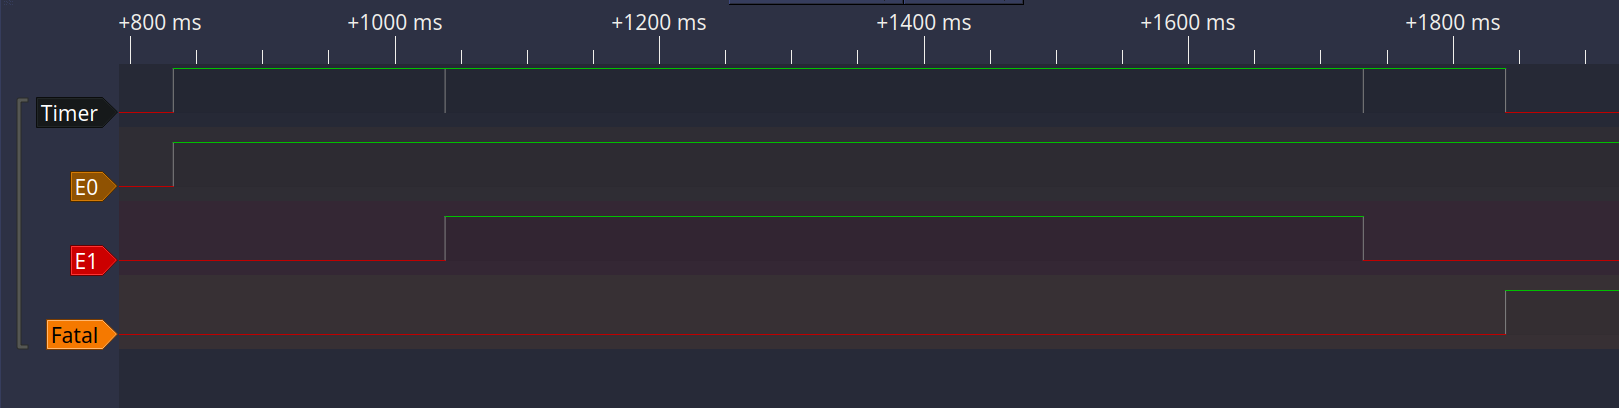
\includegraphics[width=\textwidth]{error_test}
	\caption{Error timing test. $E_1$ is reset before triggering, and the timer switches back to $E_0$.}
	\label{fig:error_test}
\end{figure}
\newpage


\chapter{Conclusions and future works}

\section{Cell Balancing}

After one hour of balancing the voltages on the segment were converging to the wanted maximum value of 3.908V. In the following hour, the algorithm was able to balance the pack to the situation seen in \autoref{fig:fenice_balanced} the state machine went into the \textit{Off} state as expected. More tests are being conducted with different balancing thresholds and discharging periods to assess the reliability of the algorithm.

Potentially harmful behavior can happen if, inside the discharging period, a cell's voltage drops below the minimum voltage cell. This occurrence can start a loop that alternately discharges all cells until undervoltage protections kick in. To avoid this problem short discharging periods are preferred along with not using too small values for the threshold. A future solution would monitor voltages continuously and stop the discharge when the voltage falls inside the threshold, without risking over-discharge the cell.

\section{Error Management}
Overall, the system works as expected and it already helped in troubleshooting while developing the firmware. There are concerns about the dynamic nature of the linked list library used as a data store. While the library is well tested and has proven to work as designed, it is generally agreed that in safety-critical applications static allocation is preferred.

There are plans to convert the error management system to a static storage solution by creating arrays of error instances that cover all the possible errors. There is a minor concern about the memory occupied by this solution since all possible errors are always allocated in RAM. However, given the characteristics of the mainboard's microcontroller \cite{f446re}, RAM is plenty for this application and no problems are expected with the current amount of errors. In any case, if memory issues arise they will be noticed at compile-time, since the whole codebase is statically allocated, so catastrophic failures at runtime are prevented.

\section{State of charge estimation}
Work is underway to implement a state of charge (SoC) estimation algorithm based around cell open-circuit voltage estimation \cite{soc}.
An important component of many commercial battery management systems is a state of charge estimation. This feature tries to guess the amount of remaining energy in each battery cell by analyzing the load current applied to the battery and its voltage to estimate the internal resistance at each instant. If the internal resistance is known, the open-circuit voltage (OCV) of the cell can be calculated using Ohm's law. With this data, SoC can be easily estimated by comparing the OCV to a voltage vs. energy function to get the remaining energy in the cell. The function can be found on the manufacturer's datasheet or can be measured with a controlled discharge of single cells.

This complex feature will be the basis of other advanced functionalities such as range estimation that can prove useful during the endurance event and power limits on lower values of SoC to prevent undervoltages and keep the battery running as long as possible.




\endgroup


% bibliografia in formato bibtex
%
% aggiunta del capitolo nell'indice
\addcontentsline{toc}{chapter}{Bibliography}
% stile con ordinamento alfabetico in funzione degli autori
\bibliographystyle{plain}
\bibliography{biblio}
%%%%%%%%%%%%%%%%%%%%%%%%%%%%%%%%%%%%%%%%%%%%%%%%%%%%%%%%%%%%%%%%%%%%%%%%%%
%%%%%%%%%%%%%%%%%%%%%%%%%%%%%%%%%%%%%%%%%%%%%%%%%%%%%%%%%%%%%%%%%%%%%%%%%%
%% Nota
%%%%%%%%%%%%%%%%%%%%%%%%%%%%%%%%%%%%%%%%%%%%%%%%%%%%%%%%%%%%%%%%%%%%%%%%%%
%% Nella bibliografia devono essere riportati tutte le fonti consultate 
%% per lo svolgimento della tesi. La bibliografia deve essere redatta 
%% in ordine alfabetico sul cognome del primo autore. 
%% 
%% La forma della citazione bibliografica va inserita secondo la fonte utilizzata:
%% 
%% LIBRI
%% Cognome e iniziale del nome autore/autori, la data di edizione, titolo, casa editrice, eventuale numero dell’edizione. 
%% 
%% ARTICOLI DI RIVISTA
%% Cognome e iniziale del nome autore/autori, titolo articolo, titolo rivista, volume, numero, numero di pagine.
%% 
%% ARTICOLI DI CONFERENZA
%% Cognome e iniziale del nome autore/autori (anno), titolo articolo, titolo conferenza, luogo della conferenza (città e paese), date della conferenza, numero di pagine. 
%% 
%% SITOGRAFIA
%% La sitografia contiene un elenco di indirizzi Web consultati e disposti in ordine alfabetico. 
%% E’ necessario:
%%   Copiare la URL (l’indirizzo web) specifica della pagina consultata
%%   Se disponibile, indicare il cognome e nome dell’autore, il titolo ed eventuale sottotitolo del testo
%%   Se disponibile, inserire la data di ultima consultazione della risorsa (gg/mm/aaaa).    
%%%%%%%%%%%%%%%%%%%%%%%%%%%%%%%%%%%%%%%%%%%%%%%%%%%%%%%%%%%%%%%%%%%%%%%%%%
%%%%%%%%%%%%%%%%%%%%%%%%%%%%%%%%%%%%%%%%%%%%%%%%%%%%%%%%%%%%%%%%%%%%%%%%%%


\titleformat{\chapter}
{\normalfont\Huge\bfseries}{Appendix \thechapter}{1em}{}
% sezione Allegati - opzionale
\appendix
\chapter{Discharge energy}
\label{chap:vtc5}
\begin{figure}[h]
	\centering
	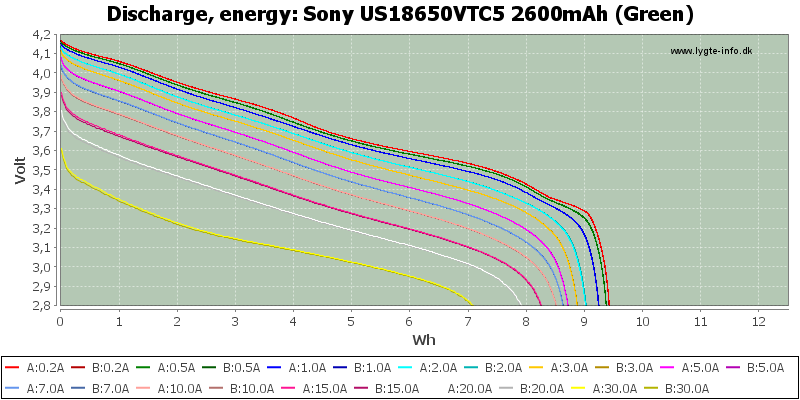
\includegraphics[scale=0.6]{pictures/vtc5.png}
	\caption{Discharge voltage vs. energy for Sony US18650VTC5 cells \cite{vtc5}}
	\label{fig:vtc5}
\end{figure}

\chapter{Balancing test}
\begin{figure}[h]
	\centering
	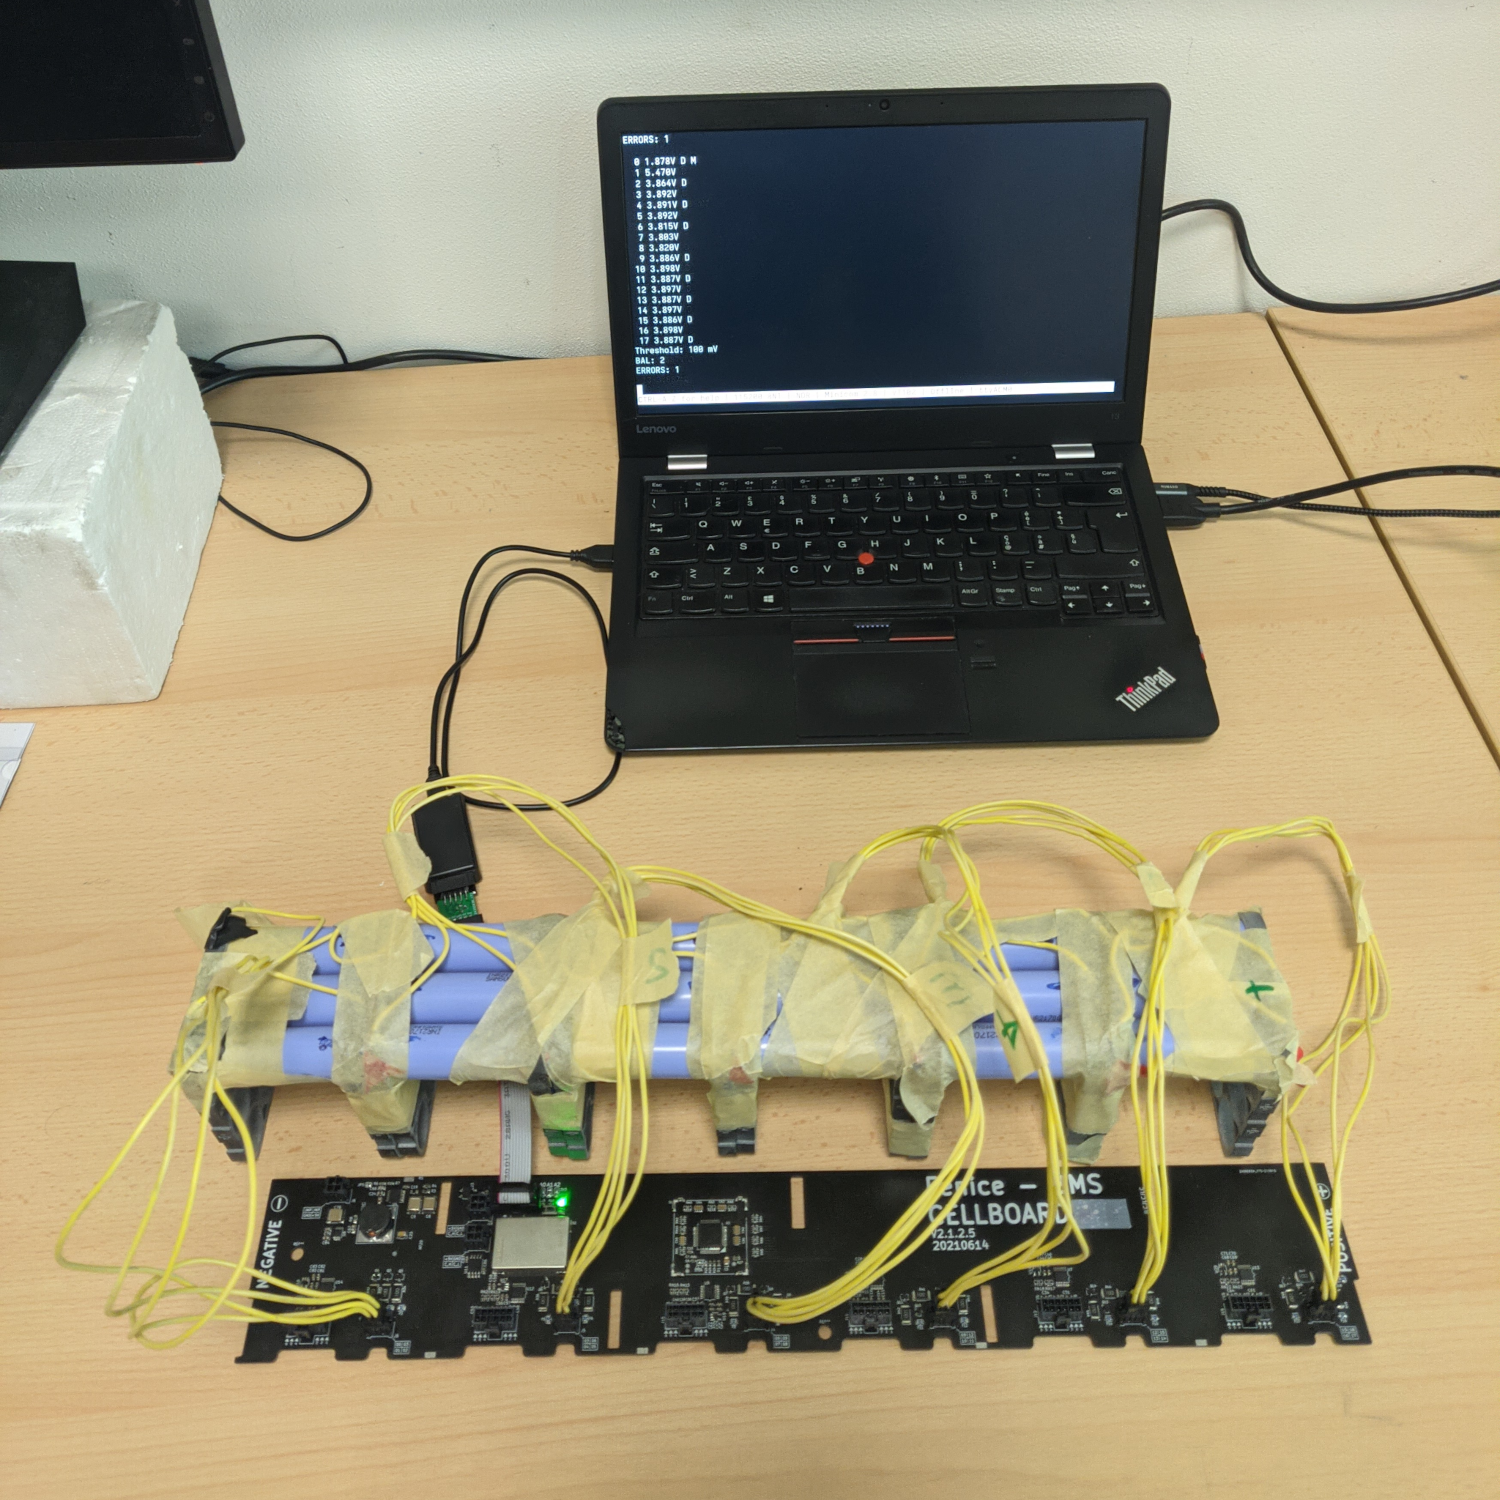
\includegraphics[scale=0.25]{balancing_test.png}
	\caption{Cell balancing test setup.}
	\label{fig:balancing_test}
\end{figure}
\begin{figure}[h]
	\centering
	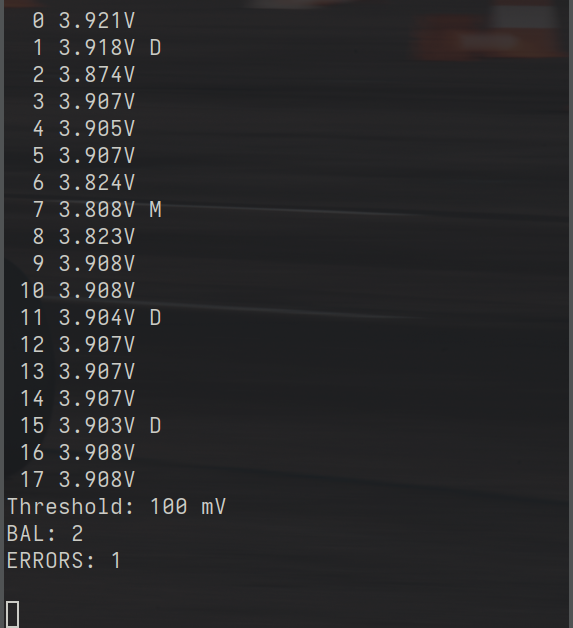
\includegraphics[scale=0.5]{balancing_console}
	\caption{Serial console during balancing. \texttt{M} indicates the minimum voltage, cells marked with \texttt{D} are being discharged}
	\label{fig:balancing_console}
\end{figure}

\chapter{Error management test}
\begin{figure}[h]
	\centering
	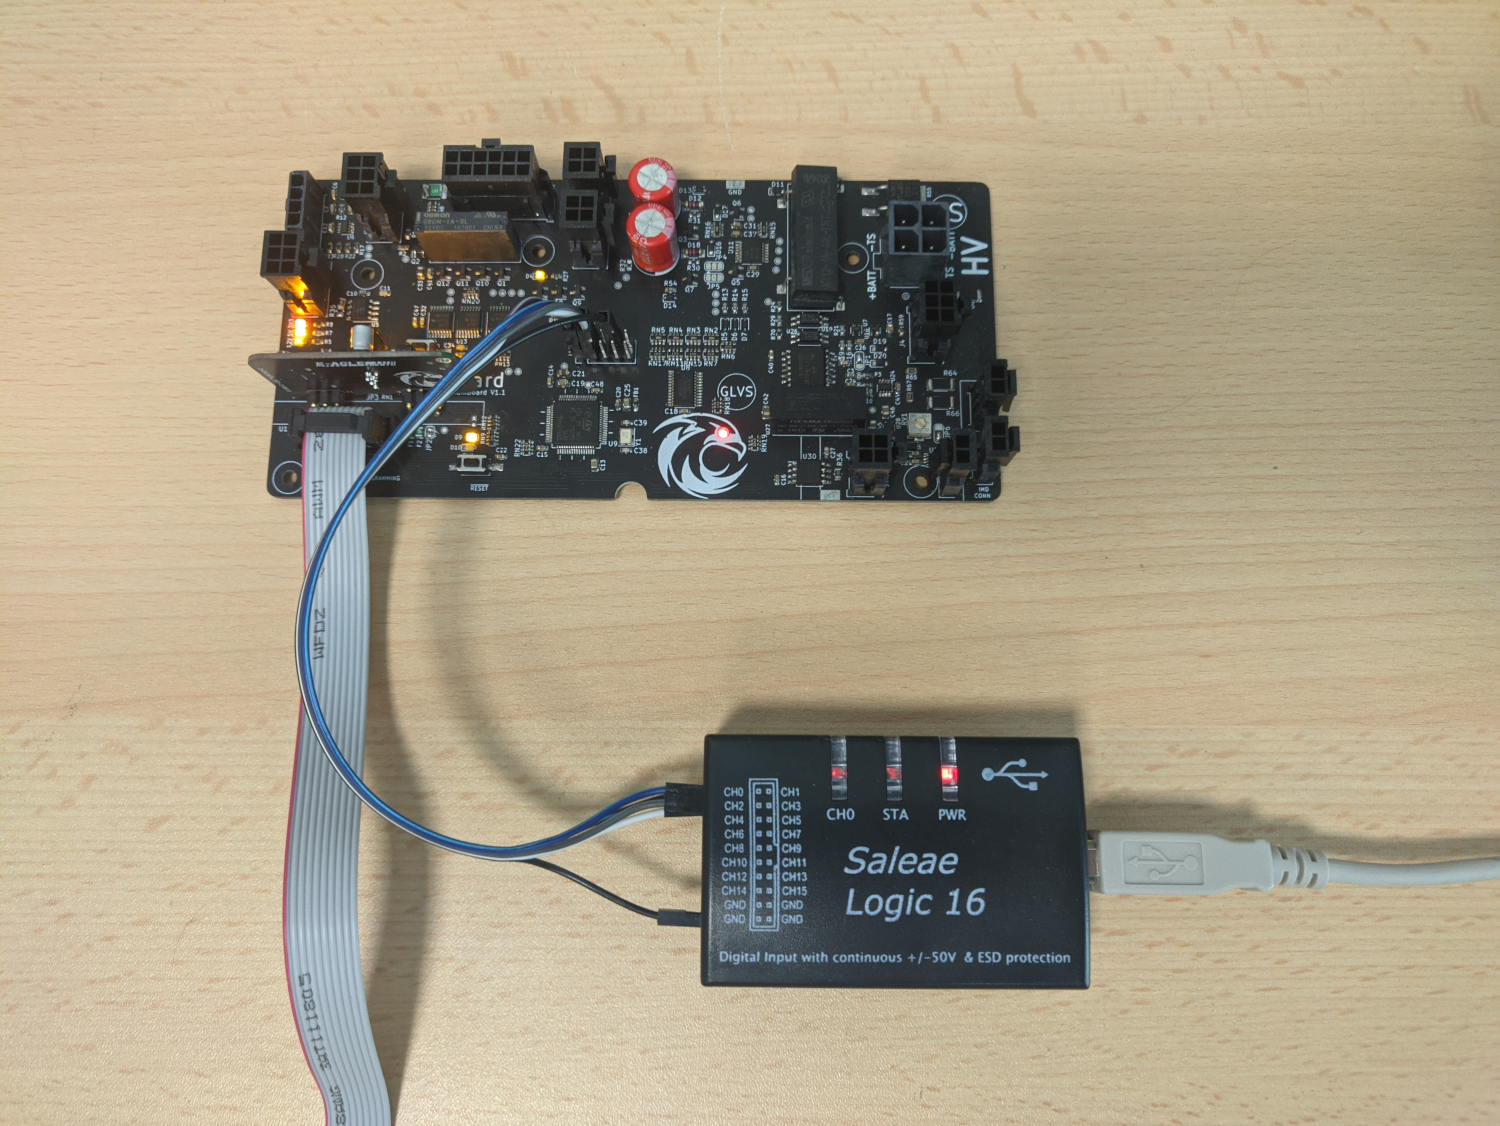
\includegraphics[scale=0.27]{error_test_setup.png}
	\caption{Error test setup with the mainboard and a logic analyzer.}
	\label{fig:error_test_setup}
\end{figure}
\begin{figure}[h]
	\centering
	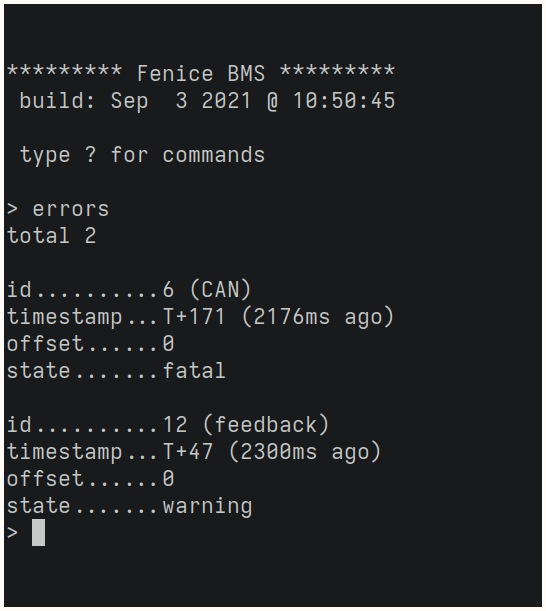
\includegraphics[scale=0.5]{error_console}
	\caption{Serial console reporting active errors.}
	\label{fig:error_console}
\end{figure}

\end{document}

